\documentclass[dvipdfmx, tikz]{standalone}

\usepackage{ifthen}

\usetikzlibrary{backgrounds}
\usetikzlibrary{arrows.meta}
\usetikzlibrary{shapes.multipart}
\usetikzlibrary{calc}

\begin{document}
  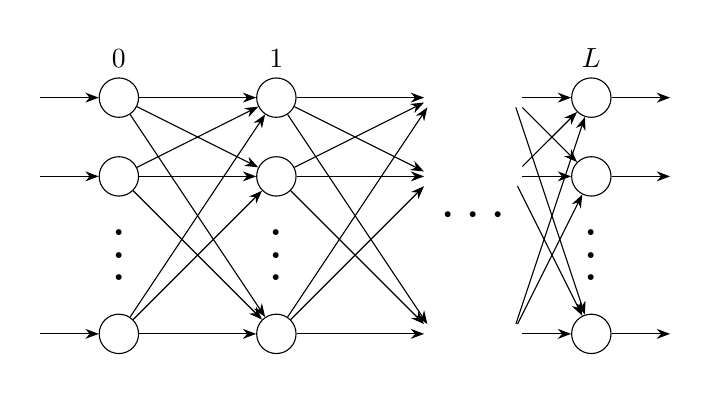
\begin{tikzpicture}[
    background rectangle/.style={fill=white},
    show background rectangle,
    neuron/.style={draw, circle, minimum width=0.5cm},
    >=Stealth, every node/.style={shape border uses incircle}]

    \def\ysep{1cm}
    \def\xsep{2cm}

    \foreach \l/\lpos/\label in {1/1/$0$, 2/2/$1$, 3/3/, 4/4/$L$} {
      \pgfmathsetlengthmacro{\lposx}{(\lpos - 1) * \xsep}
      \ifthenelse{\l=3}
      {
        \foreach \j/\jpos in {1/1, 2/2, 3/4} {
          \node (p\l\j) at (\lposx, {(-\jpos + 1) * \ysep}) {};
        }
      }
      {
        \foreach \j/\jpos in {1/1, 2/2, 3/4} {
          \node [neuron] (p\l\j) at (\lposx, {(-\jpos + 1) * \ysep}) {};
        }
        \node [scale=2, yshift=3] at ({\lposx}, -2 * \ysep) {$\vdots$};
        \node at (\lposx, 0.5*\ysep) {\label};
      }
    }

    \pgfmathsetlengthmacro{\lposx}{(3.5 - 1) * \xsep}
    \foreach \j/\jpos in {1/1,2/2, 3/4} {
        \foreach \k in {1,2,3} {
          \node (tmp) at (\lposx, {(-\jpos + 1) * \ysep}) {};
          \draw [->]  (tmp) -- (p4\k);
        }
    }


    \foreach \l/\ll in {1/2,2/3} {
      \foreach \j in {1,2,3} {
        \foreach \k in {1,2,3} {
          \draw [->] (p\l\j) -- (p\ll\k);
        }
      }
    }

    \foreach \j in {1,2,3} {
      \draw [<-] (p1\j) -- ++(-1cm, 0);
      \draw [->] (p4\j) -- ++(1cm, 0);
    }

    \pgfmathsetlengthmacro{\lposx}{(3.25 - 1) * \xsep}
    \node [scale=2] at (\lposx, {(-2.5 + 1) * \ysep}) {$\cdots$};
    
  \end{tikzpicture}
\end{document}
